\section{Vulnerability Assessment}
We are going to provide the results for each host on which the assessment was performed through \textbf{openVAS}, divided by subnet. We are going to adopt the \textbf{Severity Score} provided by \textbf{openVAS} for each of the vulnerabilities - on a scale from 0 to 10, each vulnerability is assigned a value that ranges in \textbf{None, Low, Medium, High} to describe its risk level. These values, along with their \textbf{Quality of Detection} score and the context, are then exploited to prioritize the most severe vulnerabilities in the \textbf{Analysis} subsection,where the vulnerabilities identified are discussed and mitigations are provided.\\
Every assessment was carried out requiring a minimum \textbf{QoD} of 70$\%$: we need to keep this in mind, since this minimum value, when met, means that the remote detection performed is not fully reliable.\\
Also, please notice that we are omitting several other information that \textbf{openVas} classified with severity score \textbf{Log} - 0.0. The only purpose of these information is to point out the results of different tests carried out by the tool that do not highlight vulnerabities by themselves, but are useful in the whole process and to us, as analyst, to check how the \textit{discovery, port scan, service detection and OS detection} phases were carried out by \textbf{openVAS}: some examples of these activities may be the execution of the \textbf{traceroute} command, \textbf{OS fingerprinting} operations, the \textbf{Services} log which points out all the services that were detected on the machine, \textbf{SSH} detection with corresponding algorithms to perform \textbf{encryption} and scans to determine which \textbf{cryptographic protocols} are exploited on the machine to perform \textbf{SSL/TLS}.\\
For each machine, the vulnerabilities to prioritize are highlighted in \textbf{bold}.

\subsection{Results}
\subsubsection{Internal Servers}
\textbf{DC machine - 100.100.1.2}
\begin{itemize}
\item \textbf{SSL/TLS Missing Secure Cookie Attribute - Severity Score: Medium};
\item \textbf{Missing httpOnly Cookie Attribute - Severity Score: Medium};
\item \textbf{SSL/TLS Certificate Signed Using A Weak Signature Algorithm - Severity Score: Medium};
\item TCP Timestamps - Severity Score: Low;
\end{itemize}
\begin{figure}[!htb]
\centering
\begin{minipage}{.5\textwidth}
  \centering
  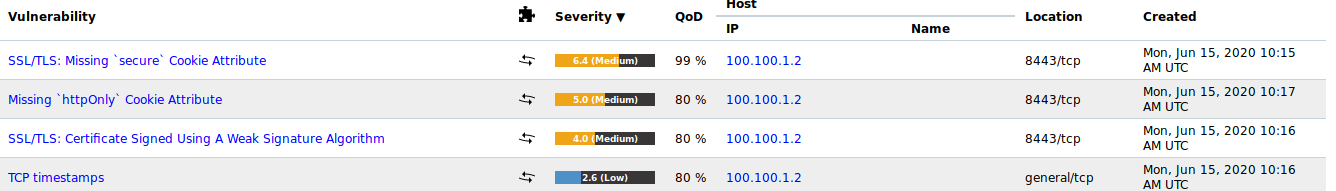
\includegraphics[width=1\textwidth]{dcVulns.png}
  \caption[a]{Vulnerabilities detected in the DC machine.}\label{fig:3}
\end{minipage}%
\end{figure}

\textbf{Log Server Machine - 100.100.1.3}
\begin{itemize}
\item TCP Timestamps - Severity Score: Low;
\end{itemize}
\begin{figure}[!htb]
\centering
\begin{minipage}{.5\textwidth}
  \centering
  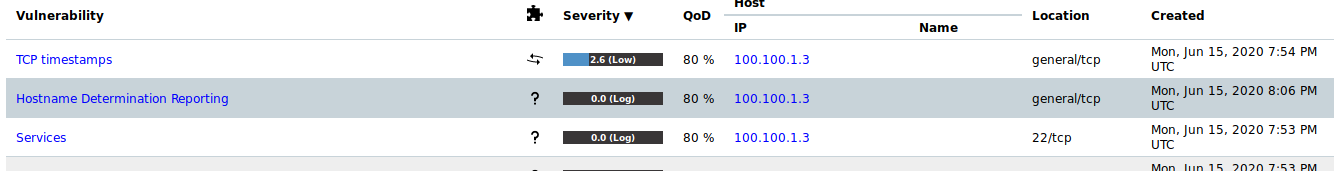
\includegraphics[width=1\textwidth]{logServerVulns.png}
  \caption[a]{Vulnerabilities detected in the Log Server machine.}\label{fig:4}
\end{minipage}%
\end{figure}

\textbf{GSM machine - 100.100.1.4}
\begin{itemize}
\item SSL/TLS: Untrusted Certificate Authorities - Severity Score: Medium;
\end{itemize}
\begin{figure}[!htb]
\centering
\begin{minipage}{.5\textwidth}
  \centering
  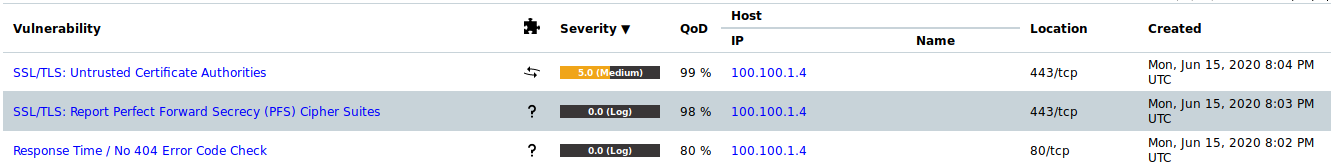
\includegraphics[width=1\textwidth]{GSM_vulns.png}
  \caption[a]{Vulnerabilities detected in the GSM machine.}\label{fig:5}
\end{minipage}%
\end{figure}

\subsubsection{Firewalls}
\textbf{Internal Firewall}
\begin{itemize}
\item \textbf{Cleartext Transmission of Sensitive Information via HTTP - Severity Score: Medium};
\item TCP timestamps - Severity Score: Low;
\end{itemize}
\begin{figure}[!htb]
\centering
\begin{minipage}{.5\textwidth}
  \centering
  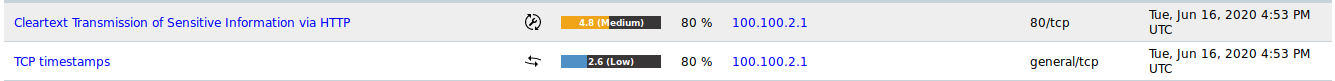
\includegraphics[width=1\textwidth]{internalFirewallVulns.png}
  \caption[a]{Vulnerabilities detected in the Internal Firewall machine.}\label{fig:6}
\end{minipage}%
\end{figure}

\textbf{Main Firewall}
\begin{itemize}
\item \textbf{Cleartext Transmission of Sensitive Information via HTTP - Severity Score: Medium};
\item TCP timestamps - Severity Score: Low;
\end{itemize}
\begin{figure}[!htb]
\centering
\begin{minipage}{.5\textwidth}
  \centering
  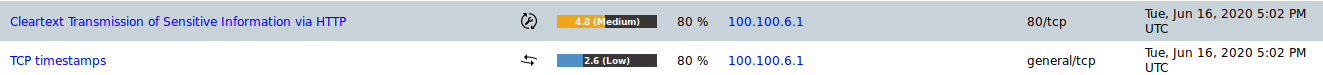
\includegraphics[width=1\textwidth]{mainFirewallVulns.png}
  \caption[a]{Vulnerabilities detected in the Main Firewall machine.}\label{fig:7}
\end{minipage}%
\end{figure}

\subsubsection{DMZ}
\textbf{Web Server Machine - 100.100.6.2}
\begin{itemize}
\item TCP timestamps - Severity Score: Low;
\end{itemize}
\begin{figure}[!htb]
\centering
\begin{minipage}{.5\textwidth}
  \centering
  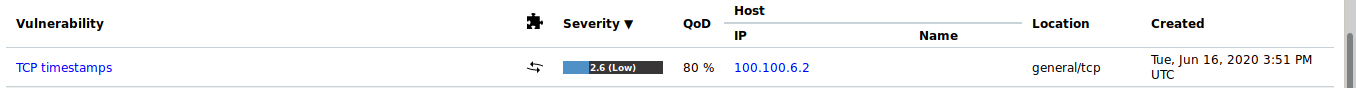
\includegraphics[width=1\textwidth]{webServerVulns.png}
  \caption[a]{Vulnerabilities detected in the Web Server machine.}\label{fig:8}
\end{minipage}%
\end{figure}

\textbf{Proxy Machine - 100.100.6.3}
\begin{itemize}
\item \textbf{SSL/TLS Missing Secure Cookie Attribute - Severity Score: Medium};
\item \textbf{Missing httpOnly Cookie Attribute - Severity Score: Medium};
\item \textbf{SSL/TLS Certificate Signed Using A Weak Signature Algorithm - Severity Score: Medium};
\item TCP Timestamps - Severity Score: Low;
\end{itemize}
\begin{figure}[!htb]
\centering
\begin{minipage}{.5\textwidth}
  \centering
  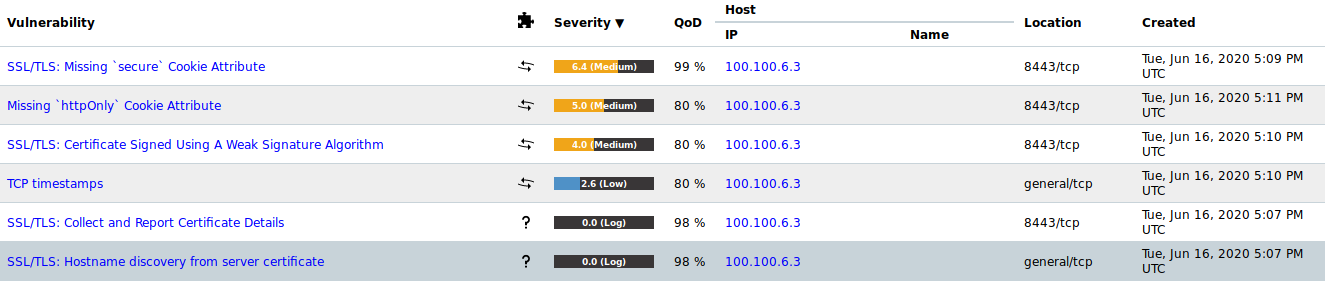
\includegraphics[width=1\textwidth]{proxyVulns.png}
  \caption[a]{Vulnerabilities detected in the Proxy machine.}\label{fig:9}
\end{minipage}%
\end{figure}

\subsection{Analysis}

Obviously, the fact that machines implementing the same services - \textbf{DC} and \textbf{Proxy} with \textbf{Zentyal}, both \textbf{firewalls} with \textbf{OPNSense} - were also diagnosed with the same vulnerabilities, is not simply due to chance. This is an advantage, since when we know how to fix a vulnerability in one of those machines, we also know how to fix it in the other one. We are thus now analyzing one by one the prioritized vulnerabilities - aslo explaining \textit{why} we chose to prioritize them - and then those that are left.\\

\subsubsection{Cleartext Transmission of Sensitive Information via HTTP}
\begin{itemize}
\item Severity Score: \textbf{Medium};
\item Affected Machines: Internal Firewall, Main Firewall (OPNSense);
\end{itemize}
\begin{figure}[!htb]
\centering
\begin{minipage}{.5\textwidth}
  \centering
  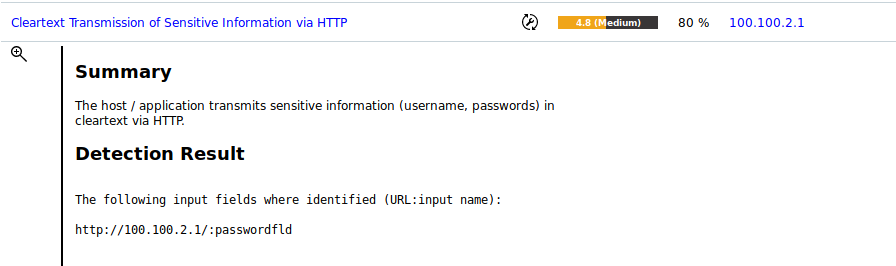
\includegraphics[width=1\textwidth]{clearTextHTTPfirewallVuln.png}
  \caption[a]{Password is sent in cleartext through HTTP.}\label{fig:10}
\end{minipage}%
\end{figure}

One of the desired features of a Firewall, is that of being immune to penetration. Firewalls are the first devices we should protect in our network, as they filter the traffic that is destined in/out from our subnetworks, and they also implement several other services (DHCP, suricata, OpenVPN...). Not to mention their importance in routing. This vulnerability affects the \textbf{OPNSense} service, and is due to the fact that \textbf{HTTPS} is not enabled.\\
This is probably the most important vulnerability to mitigate due to its potentially huge negative impact on our network and to the relatively easy fix.\\
Suggested way to mitigate this is indeed by checking at both firewalls the \textbf{HTTPS} box on option \textbf{Protocol} under \textit{System $->$ Settings $->$ Administration} as pictured in \textbf{Figure 11}: this way, authentication parameters - as well as any other data - should be sent through an encrypted channel. Since an adversary sniffing the devices' traffic might have already exploited this vulnerability, once mitigated it is also recommended to at least change all the passwords for each user in both firewalls.

\begin{figure}[!htb]
\centering
\begin{minipage}{.5\textwidth}
  \centering
  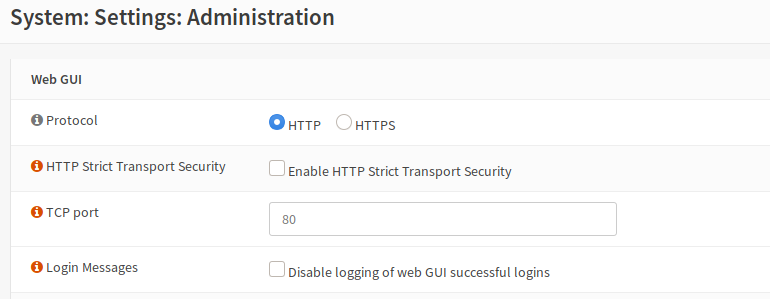
\includegraphics[width=1\textwidth]{vulnerabilityToMitigate.png}
  \caption[a]{Suggested fix.}\label{fig:11}
\end{minipage}%
\end{figure}

\subsubsection{SSL/TLS Certificate Signed Using A Weak Signature Algorithm}
\begin{itemize}
\item Severity Score: \textbf{Medium};
\item Affected Machines: DC, Proxy (Zentyal);
\end{itemize}
\begin{figure}[!htb]
\centering
\begin{minipage}{.5\textwidth}
  \centering
  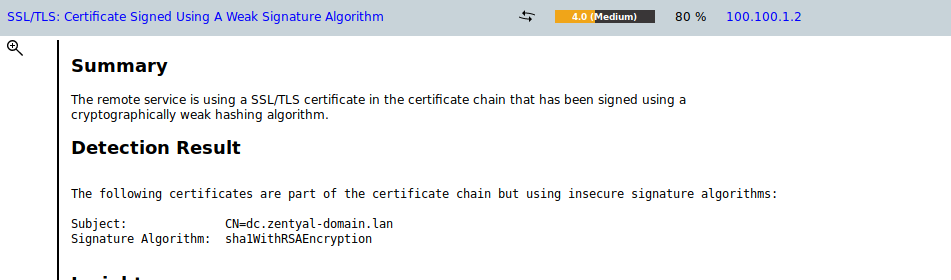
\includegraphics[width=1\textwidth]{weakSHA1CertificateDCVuln.png}
  \caption[a]{Certificate is signed with a weak algorithm - SHA1.}\label{fig:14}
\end{minipage}%
\end{figure}

The certificate provided for SSL/TLS sessions by both the machines is signed through \textbf{SHA-1 algorithm}, which is publicly known to be, nowadays, \textbf{not secure}, due to the fact that in 2017 the \textbf{Google Security Team} announced to have broken the algorithm by finding a collision. This means the certificate can be forged, it is possible to impersonate both machines and a \textit{MITM} attack is technically feasible on them. To mitigate this threat, it is recommended to generate a new certificate, one for each service running in the two machines, signed with a different algorithm, e.g. \textbf{SHA-250} or \textbf{SHA-3}. We do not know, though, whether this fix can be applied directly by us or it requires the vendor of the product.

\subsubsection{SSL/TLS Missing Secure Cookie Attribute}
\begin{itemize}
\item Severity Score: \textbf{Medium};
\item Affected Machines: DC, Proxy (Zentyal);
\end{itemize}
\begin{figure}[!htb]
\centering
\begin{minipage}{.5\textwidth}
  \centering
  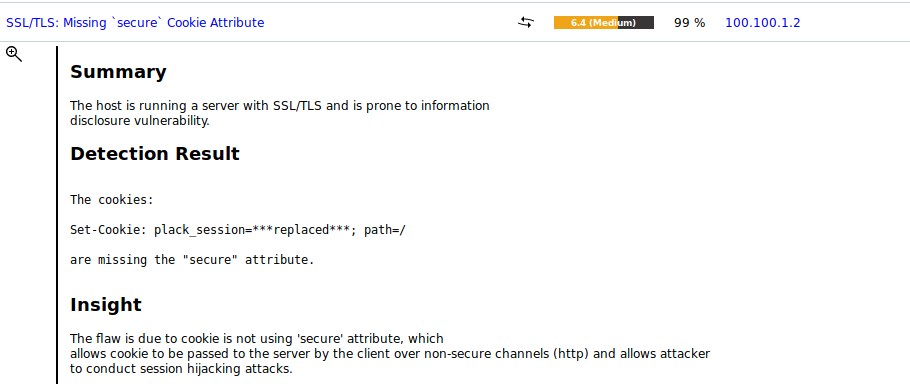
\includegraphics[width=1\textwidth]{secureCookiesDCVuln.png}
  \caption[a]{Cookies could be sent through an unencrypted channel.}\label{fig:12}
\end{minipage}%
\end{figure}

\textbf{Zentyal} service, reachable at port \textbf{8443} in both machines, already exploits the \textbf{HTTPS} protocol, so the server is running with \textbf{SSL/TLS}, but the \textit{Secure} flag is not sent for the cookies that may be used to remember an already authenticated user - meaning the cookies could be sent in clear text. This would allow an adversary which sniffs the traffic to read the cookie an authenticated client sends to the server, if the client sends it through an unencrypted channel, and exploit it to \textit{hijack his session} and be authenticated by \textbf{Zentyal} as an user with privileges, potentially leading to a disruption of the services running in the machines. We found no ways to actually instruct \textbf{Zentyal} on which cookies to accept and with which parameters - this might be a feature only available in the commercial edition, or only to the vendor of the product itself.\\
Beacuse of this, our only way to mitigate this vulnerability may be to make sure that no adversary is able to join the subnetworks of the two \textbf{Zentyal} machines and perform eavesdropping.

\subsubsection{Missing httpOnly Cookie Attribute}
\begin{itemize}
\item Severity Score: \textbf{Medium};
\item Affected Machines: DC, Proxy (Zentyal);
\end{itemize}
\begin{figure}[!htb]
\centering
\begin{minipage}{.5\textwidth}
  \centering
  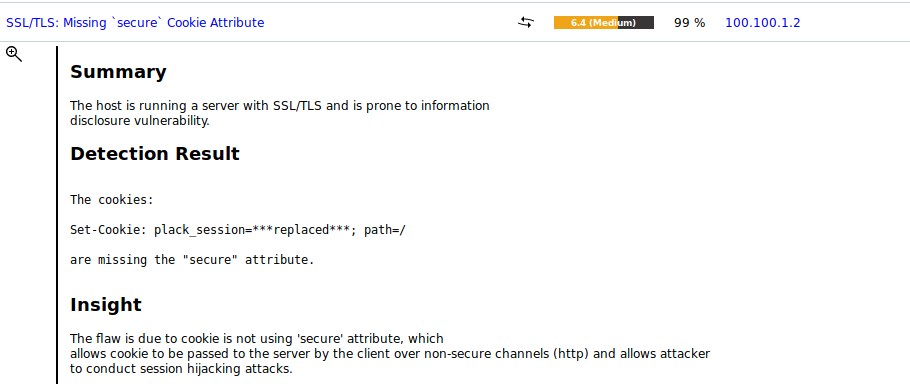
\includegraphics[width=1\textwidth]{secureCookiesDCVuln.png}
  \caption[a]{Cookies can be accessed through JavaScript code.}\label{fig:13}
\end{minipage}%
\end{figure}

This vulnerability is similar to the previous one, except it describes the cookies set by \textbf{Zentyal} to be missing the \textbf{httpOnly} attribute. This flag in a cookie prevents it from being accessed by scripts at client side - e.g. a JavaScript script accessing the cookie through the DOM of the web page. Just like the previous vulnerability, this might lead to \textit{session hijacking} as a result of \textit{XSS attacks}.\\
The only way to mitigate this vulnerability is the one we already highlighted in the previous subsection about \textbf{SSL/TLS Missing Secure Cookie Attribute} vulnerability.

\subsubsection{Low priority vulnerabilities}

\textbf{1. SSL/TLS: Untrusted Certificate Authorities}
\begin{itemize}
\item Severity Score: \textbf{Medium};
\item Affected Machines: GSM;
\end{itemize}
\begin{figure}[!htb]
\centering
\begin{minipage}{.5\textwidth}
  \centering
  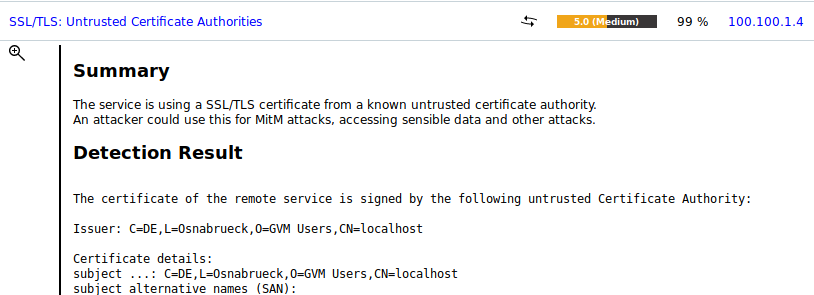
\includegraphics[width=1\textwidth]{certificateUntrustedAuthorityTLSGSM.png}
  \caption[a]{GSM - untrusted CA.}\label{fig:14}
\end{minipage}%
\end{figure}
This is probably a minor, false alarm: the CA signing the certificate for the \textit{GSM} machine is \textbf{Greenbone} itself, the scanner doesn't recognize it as a public, trustworthy CA, but we as users know it can be trusted.\\

\textbf{2. TCP timestamps}
\begin{itemize}
\item Severity Score: \textbf{Low};
\item Affected Machines: all, except GSM machine;
\end{itemize}
\begin{figure}[!htb]
\centering
\begin{minipage}{.5\textwidth}
  \centering
  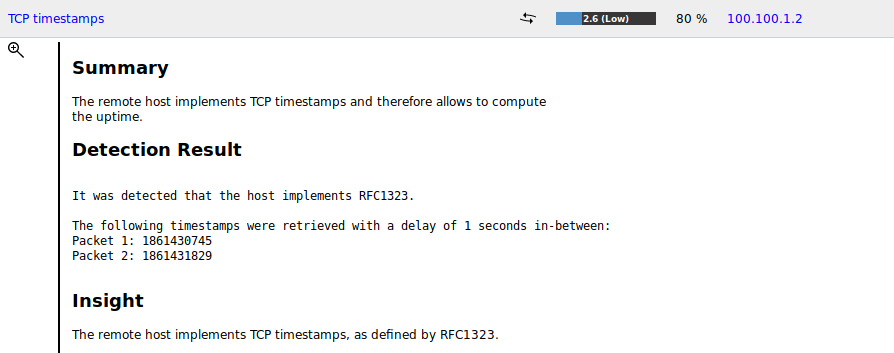
\includegraphics[width=1\textwidth]{tcpTimestampsVuln.png}
  \caption[a]{TCP Timestamps vulnerability in DC machine.}\label{fig:15}
\end{minipage}%
\end{figure}
\textbf{TCP timestamps} allow to compute the uptime of each host in the network. This provides extra information to an attacker, such as knowing when was the last time the machine was rebooted - which is something that occurs likely, for example, to install patches and updates. This might lead adversary to guess whether the system has installed the latest patches and updates, which might provide protection against latest exploits found on the system, or not, as well as to other exploits. However, hiding \textbf{TCP timestamps} for these reasons is basically \textit{security through obscurity}, which is commonly known to be a bad practice: real protection should be provided by always checking periodically the last updates and patches, and install them.\\
If needed, mitigation is provided by \textbf{openVAS} itself in the picture below, and can be easily applied to all the machines - but this might need further analysis, since disabling the TCP timestamps may also affect the system's performances as well as disable some other security features (see next section).\\
\begin{figure}[!htb]
\centering
\begin{minipage}{.7\textwidth}
  \centering
  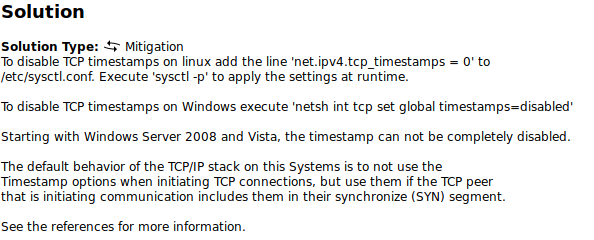
\includegraphics[width=1\textwidth]{tcpTimestampsVulnMitigation.png}
  \caption[a]{TCP Timestamps mitigation.}\label{fig:16}
\end{minipage}%
\end{figure}
